\documentclass[a4paper,12pt]{article}
%usepackgae
\usepackage[utf8]{vietnam}
\usepackage{amssymb}
\usepackage{amsmath}
\usepackage{amsfonts}
\usepackage{graphicx}
%title
\title{\vspace{-8ex} \bfseries Trực giác về phép tính Giới hạn qua các bài toán kinh điển}
\date{\vspace{-8ex}}

\begin{document}
\maketitle
\textbf{1. Bài toán tìm hệ số góc tiếp tuyến của Fermat}\\

Lý luận giải quyết bài toán của Fermat:

\begin{center}
	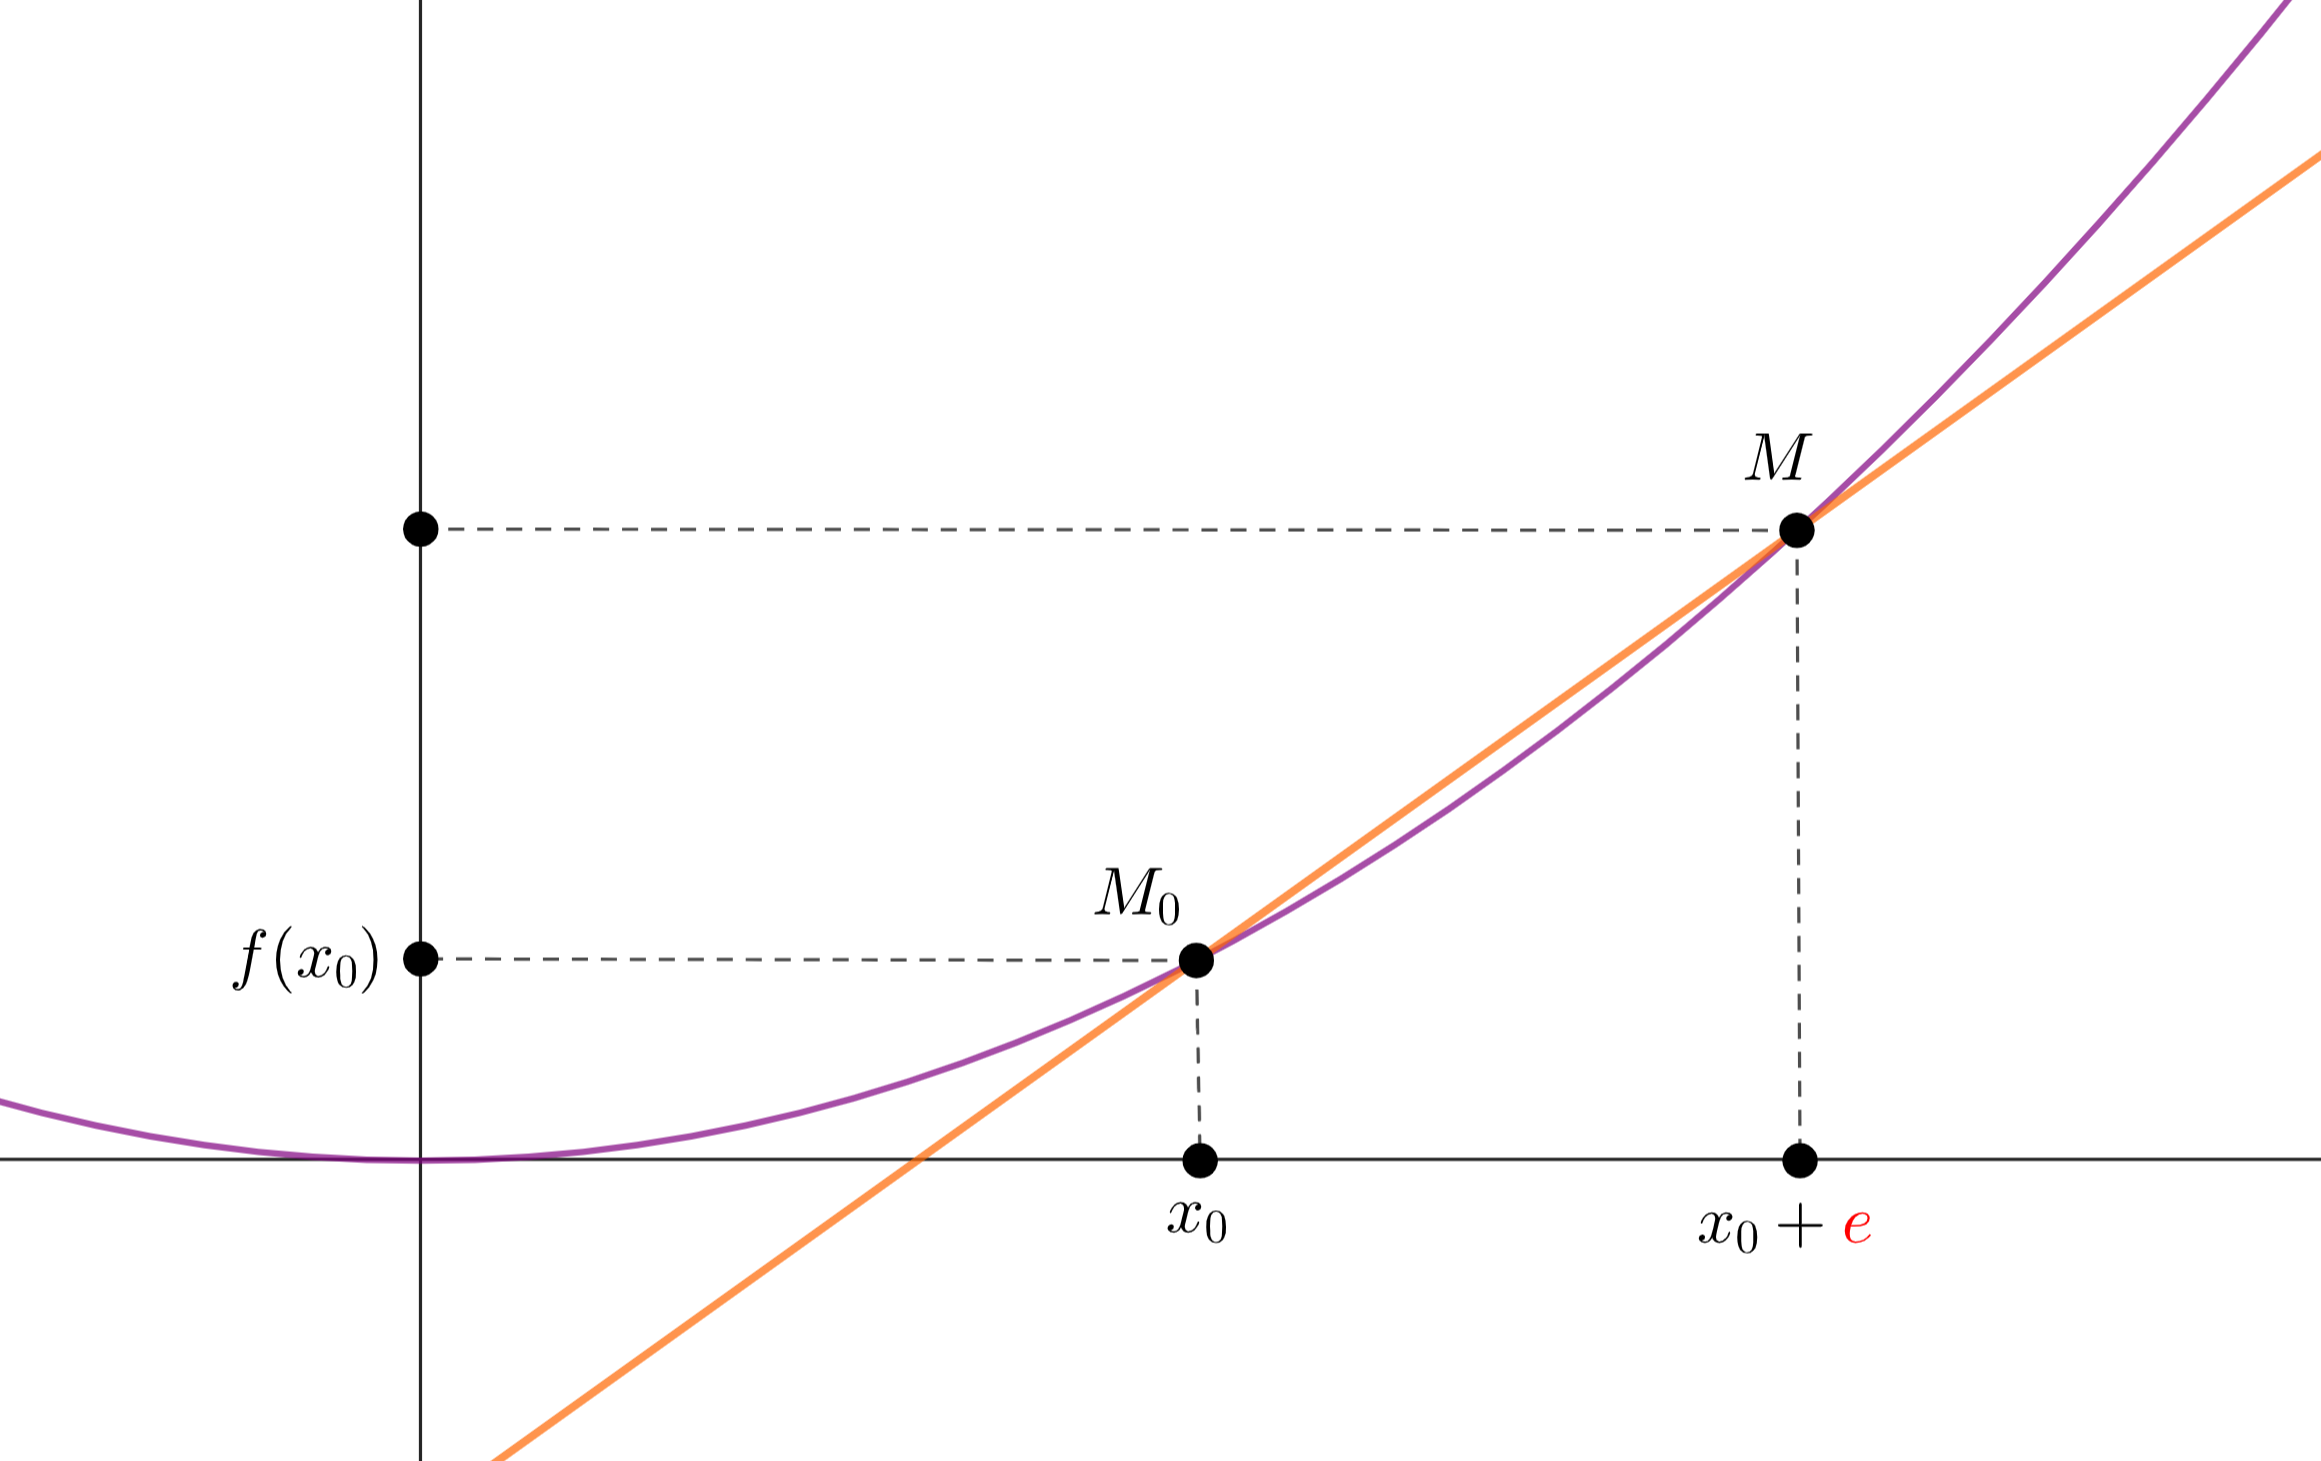
\includegraphics[width=0.8\textwidth]{fermat}\\
	\textit{hình 1.1}
\end{center}

Trên đường cong cho bởi hàm số $y=f(x)$, giả sử có thêm một điểm trên đường cong có khoảng cách hoành độ với hoành độ tiếp điểm $M_0$ của tiếp tuyến là \footnote{$e$: đại lượng vô cùng bé (infinitesimal)}$e$, hai điểm này gần nhau vô hạn nhưng là hai điểm phân biệt, vì vậy xem đường cát tuyến nối hai điểm như một tiếp tuyến \textit{(hình 1.1)}. Sau đó trong phương trình hệ số góc cát tuyến giữa hai điểm rất gần nhau như vậy, có thể khéo léo loại bỏ đi lượng $e$ (vì $e$ nhỏ đến độ có thể xem như không tồn tại) để có được hệ số góc tiếp tuyến. Giả sử cho hàm số $y=x^2$, gọi $slope$ là hệ số góc tiếp tuyến của $y$ tại $M_0$, giải pháp đại số có được:\\
$$ slope=\frac{f(x)-f(x_0)}{x-x_0} = \frac{(x_0+e)^2-x_0^2}{e}=\frac{2x_0e+e^2}{e}=2x_0+e=2x_0.$$

Có vẻ như phương pháp lý luận hình học về tiếp tuyến đường cong của Fermat là không sai và cho ra kết quả đẹp, nhưng việc sử dụng đại lượng $e$ một cách quá trực diện mà ông đã bỏ qua "tính quá trình" trong lý luận. Mấu chốt ở chỗ, giả sử nếu Fermat lập luận với lý luận hình học về tiếp tuyến đường cong có được tính quá trình như sau:\\

Trên đường cong cho bởi hàm số $y=f(x)$, cho tiếp điểm cát tuyến $M_0$ "tiến về" tiếp điểm còn lại (nhưng không trùng) cho đến khi khoảng cách hoành độ giữa chúng là một lượng $e$ (hai điểm này gần nhau vô hạn nhưng là hai điểm phân biệt, vì vậy xem đường cát tuyến nối hai điểm như một tiếp tuyến). Sau đó trong phương trình hệ số góc cát tuyến giữa hai điểm rất gần nhau như vậy, chỉ việc bỏ tất cả các lượng có chứa $e$ (vì $e$ nhỏ đến độ có thể xem như không tồn tại) để có được hệ số góc tiếp tuyến.\\

Qua lý luận có được tính quá trình như trên vừa nêu, ta có thể dễ dàng mường tượng ra được điểm $M$ đã cho, đóng vai trò như một "điểm chuyển động" trên đồ thị hàm số $y=f(x)$. Một dự đoán về "giới hạn" của quá trình "tiến về" xuất hiện qua trực giác khi các thông tin biểu hiện vị trí của một điểm theo hàm số trên bảng tính khảo sát được nhận liên tục các giá trị giả định, chúng thể hiện rằng: khi cho $x$ nhận những giá trị "càng gần" $x_0$, nếu $f(x)$ cũng "càng gần" $f(x_0)$ và gần "tùy ý" miễn là cho $x$ "đủ gần" $x_0$, thì $f(x_0)$ chính là giới hạn của hàm số $f(x)$ khi $x$ tiến về $x_0$.\\

Rõ ràng hơn, điều này cho ta hàm ý rằng với: $$slope=\frac{f(x)-f(x_0)}{x-x_0}=G(x),  \mathbf{D}=\mathbb{R}\backslash{\{x_0\}}$$ khi cho $x$ nhận những giá trị "càng gần" $x_0$, nếu $G(x)$ cũng "càng gần" một giá trị nào đó, mà ta giả sử gọi chúng là $L$ và gần "tùy ý", miễn là cho $x$ "đủ gần" $x_0$, thì $L$ được gọi là giới hạn hàm số $G(x)$ khi $x$ tiến về $x_0$.\\

Như vậy, một cách tổng quát, cho một hàm số $y=f(x)$: 
Nếu $f(x)$ có thể gần $L$ "tùy ý" ($f(x)$ tiến về $L$: $f(x) \to L$), miễn là cho $x$ "đủ gần" $x_0$ ($x$ tiến về $x_0$: $x \to x_0$), thì $L$ được gọi là Giới hạn của Hàm số $f(x)$ khi $x$ tiến về $x_0$.\\

\newpage

\textbf{2. Bài toán vận tốc tức thời của chuyển động của Newton}\\

Trong tác phẩm \textit{The Method of Fluxions (1736)}, Newton từng viết: 
\begin{quote}
	\textit{"Tôi không nghĩ rằng những vật thể toán học được tạo nên bởi những phần, dầu là rất nhỏ, mà là tạo nên bởi một sự chuyển động liên tục. Đường không phải do sự kết hợp bởi những phần của nó, mà là được tạo nên bởi một điểm chuyển động. Mặt thì do những đường chuyển động tạo thành."}
\end{quote}

Đến với bài toán, Newton gọi các đại lượng $x,y$ cấu thành một điểm chuyển động (theo thời gian $t$) trên đồ thị hàm số là $fluent$, gọi vận tốc của chúng là $fluxion$ kí hiệu $\dot{x}, \dot{y}$. Mặt khác ta có $\Delta x=v_x\Delta t$ và $\Delta y=v_y\Delta t$.\\

\begin{center}
	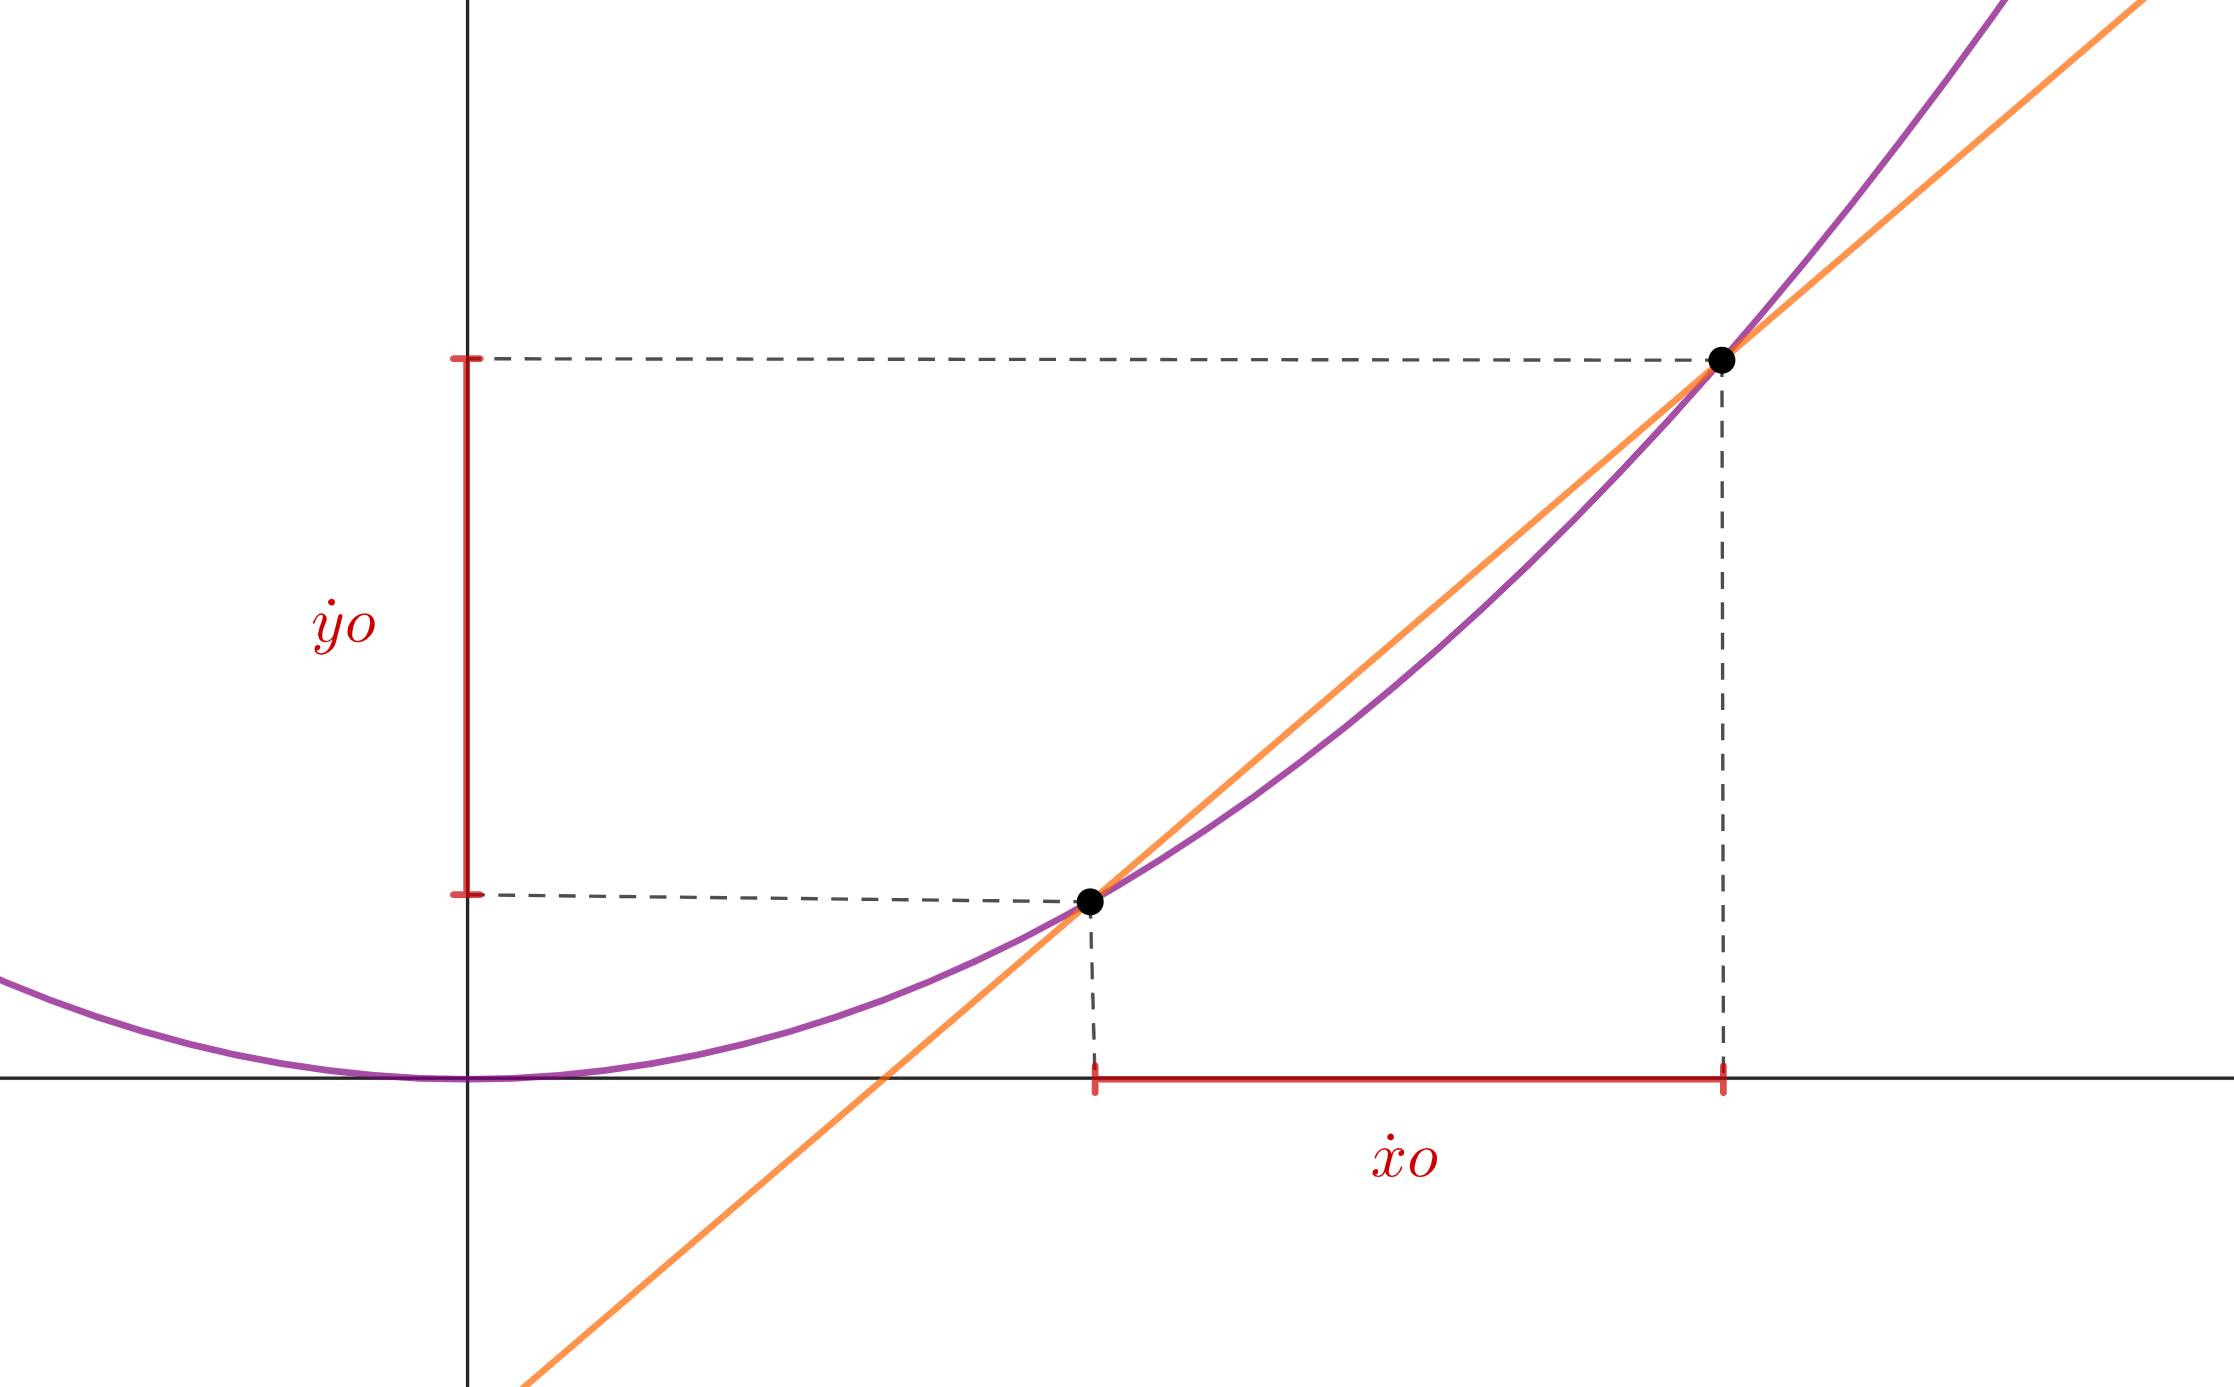
\includegraphics[width=0.8\textwidth]{newton}\\
	\textit{hình 1.2}
\end{center}
 
Xét vận tốc điểm chuyển động ở trong khoảng thời gian là $\Delta t=o$ rất bé, bé như ý tưởng của đại lượng vô cùng bé. Vì $\Delta t=o$ nên lượng thay đổi của $x, y$ khi đó cũng là vô cùng bé, có thể viết thành $\Delta x=\dot{x}o$ và $\Delta y=\dot{y}o$ \textit{(hình 1.2)}. Giả sử cho hàm số $y=x^2$, gọi $\dot{v}_x$ là vận tốc biến thiên tức thời tại $x$ của hàm $y$, giải pháp đại số có được:

$$\dot{v}_x=\frac{\dot{y}o}{\dot{x}o}=\frac{(x+\dot{x}o)^2-x^2}{(x+\dot{x}o)-x}=\frac{2x\dot{x}o+(\dot{x}o)^2}{\dot{x}o}=2x+\dot{x}o=2x$$

Trong bài toán, ta thấy Newton cũng sử dụng đến đại lượng $e$, nhưng khác với Fermat, Newton xem trọng "tính quá trình" khi lý luận phương pháp cho bài toán qua hình học với ý tưởng "điểm chuyển động". Vì vậy, Newton đã thật sự chạm đến khái niệm Giới hạn trong giải pháp cho bài toán này.\\
\newline

\textbf{3. Bài toán diện tích miền trên mặt phẳng của Leibniz}\\

Trong khi Newton tiếp cận với khái niệm Fluxion, một cách độc lập, Leibniz cũng tạo ra ý tưởng hệ số Vi phân của mình khi làm việc với bài toán diện tích miền trên mặt phẳng.\\ 

Ông gọi $dy$ là một lượng thay đổi nhỏ vô hạn của $y$ (hay Vi phân của $y$) do (tương ứng với, gây ra bởi) một lượng thay đổi nhỏ vô hạn của $x$ (hay Vi phân của $x$) để đạt được "tốc độ biến thiên tức thời của hàm $y$ tại $x$", được biểu thị bằng hệ số Vi phân: $$\frac{dy}{dx}$$

Giống với Newton, cách viết lý luận cho khái niệm Vi phân bằng các "lượng thay đổi nhỏ vô hạn" cho thấy ông cũng xem trọng "tính quá trình" biến thiên của hàm.\\

Giải pháp hoạt động gần như tương tự với khái niệm Fluxion, bằng cách dùng đại lượng $e$ giả định để xác định hệ số Vi phân, qua đó xây dựng được cơ sở tính toán thực (hiện thực hoá) cho ý tưởng Tích phân là công thức Newton-Leibniz quen thuộc ngày nay:

$$ \int_{a}^{b} f(x)dx = F(x) \Big|_{a}^{b} = F(b) - F(a) $$
với $F$ được gọi là Nguyên hàm của $f$.\\

Sau cùng, Vi phân của Leibniz cũng là một "đối tượng cơ bản" để phục vụ cho việc định nghĩa Đạo hàm. Giống với cách Archimedes, Fermat, Newton dùng $e$ để tính toán diện tích hình tròn, hệ số góc tiếp tuyến hay vận tốc tức thời của chuyển động, trở thành tiền đề sau đó cho việc định nghĩa Đạo hàm. Mặc dù theo cách hiểu hiện đại, nó không phải.\\

Vào cuối thế kỷ 19, các nhà toán học cảm thấy rằng đại lượng $e$ chứa đựng những mơ hồ và mâu thuẫn với lý thuyết đại số thuần túy trong quá trình phát triển của nó. Một số nhà toán học thế kỷ 19 (Weierstrass, Bolzano và những người khác) đã tìm ra phép tính Giới hạn với định nghĩa có hình thức $\epsilon - \delta$ chặt chẽ về mặt đại số hơn $e$ rất nhiều, trong khi Cauchy khai thác cả khái niệm $e$ và Giới hạn (xem \footnote{Sách của Augustin-Louis Cauchy (1821): Analysis Course}\textit{Cours d'Analyse} ). Tuy nhiên, ký hiệu Vi phân của Leibniz vẫn được sử dụng phổ biến vì tính kỹ thuật (ảnh hưởng nhiều đến phương pháp Tích phân đã có, điển hình trong phép biến đổi Tích phân chúng ta có thể đối phó với chúng như những ký hiệu đại số thông thường) và tính gợi ý tuyệt vời trong các tính toán, cho phép cung cấp các biểu thức gọn gàng và trực quan. Do đó ký hiệu đã được giải thích lại về mặt định nghĩa dù rằng ý tưởng của phương pháp Vi phân cho Đạo hàm không sai. Vì vậy, để thoát khỏi đó, Đạo hàm phải được định nghĩa trên phép tính Giới hạn rồi xem Đạo hàm như một "đối tượng cơ bản", còn $dy, dx$ như những giá trị đại số, với $dx$ sao cho thỏa mãn phương trình $dy=f'(x)dx$, khi đó $dy$ được gọi là Vi phân của hàm $y$ tại $x$.
\end{document}